\setchapterimage[6cm]{chapter/operating_system/logo.png}
\setchapterpreamble[u]{\margintoc}
\chapter[line 1 line 2]{Programming languages for operating systems}
\labch{operating-sysmets}

\section{Annotation}
The chapter explores the object of the <<operating system>> and its properties. The following problems were solved in the paper with the help of SPARQL queries: finding instances of the object <<operating system>>, building a list of operating systems (OS) by base, by creation time, by programming language, in which the OS was written. Also a histogram is constructed, it shows the number of programs written in some programming language, and the proportion of how many of them work for some OS. A lot of software does not specify the programming language on which it was developed. The property <<programming language>> was added to several objects to improve the results.

\section{Instances of the object "operating system"}

Let's build a list of all the operating systems.

\begin{lstlisting}[ language=SPARQL, 
caption={List of operating systems\\\hspace{\textwidth} 
SPARQL query \num{510} results (January 2018), \num{1086} results (September 2020).
SPARQL query: \href{https://w.wiki/nDb}{https://w.wiki/nDb}
},
label=lst:os-list,
texcl 
]
#List of `instances of` "operating system" 
SELECT ?os ?osLabel
WHERE
{
	?os wdt:P31 wd:Q9135.
	SERVICE wikibase:label { bd:serviceParam wikibase:language "en" }
}
}
\end{lstlisting}

[+]> The most complete and detailed operating systems on Wikidata are: Linux, Windows, Windows 8

[-]> Almost empty and less informative operating systems are: SPIN, JavaOS, Atari TOS, Xubuntu

According to ProWD the only one Russian operating system on Wikidata is Miraculix, which has 7 properties. The leaders in terms of the number of properties (24 properties) among operating systems around the world are Microsoft Windows and Windows 8.

\section{List of operating systems by base}

\begin{lstlisting}[ language=SPARQL, 
caption={List of operating systems by base\\\hspace{\textwidth}
SPARQL query \num{159} results (January 2018), \num{118} results (September 2020).
SPARQL query: \href{https://w.wiki/nDc}{https://w.wiki/nDc}
},
label=lst:os-by-base,
texcl 
]
SELECT ?osLabel ?baseLabel
WHERE
{
	?os wdt:P31 wd:Q9135. # inctance of operating system
	?os wdt:P144 ?base. # os is base for 
	SERVICE wikibase:label { bd:serviceParam wikibase:language "en" }
}
GROUP BY ?osLabel ?baseLabel
\end{lstlisting}

\section{List of operating systems by creation time}


\begin{lstlisting}[ language=SPARQL, 
caption={List of operating systems by creation time\\\hspace{\textwidth}
SPARQL query \num{298} results (January 2018), \num{238} results (September 2020).
SPARQL query: \href{https://w.wiki/nDf}{https://w.wiki/nDf}
},
label=lst:os-creation-time,
texcl 
]
#defaultView:Timeline
SELECT ?osLabel ?time
WHERE
{
	?os wdt:P31 wd:Q9135. # inctance of operating system
	?os wdt:P571 ?time. # created at
	SERVICE wikibase:label { bd:serviceParam wikibase:language "en" }
}
GROUP BY ?osLabel ?time
ORDER BY DESC(?time)
\end{lstlisting}

\section{Count of operating systems by programming language}

\begin{lstlisting}[ language=SPARQL, 
caption={Count of operating systems by programming language\\\hspace{\textwidth}
SPARQL query \num{35} results (January 2018), \num{37} results (September 2020).
SPARQL query: \href{https://w.wiki/nDh}{https://w.wiki/nDh}
},
label=lst:prog-lang-count,
texcl 
]
#defaultView:BarChart
SELECT ?lang (count(*) as ?count)
WHERE 
{
	?os wdt:P31 wd:Q9135.
	?os wdt:P277 ?langObj .
	OPTIONAL {
		?langObj rdfs:label ?lang
		filter (lang(?lang) = "en")
	}
}
GROUP BY ?lang
ORDER BY DESC(?count) ASC(?lang)
\end{lstlisting}

The query shows (only on the basis of the completed wikis, so it's not a fact that it's true) that the OS is predominantly written in Assembler language, which is certainly true, because it is the fastest, yet convenient programming language. On the second and third places are C and C++, which are not the worst analogue, because in spite of its "slowness", they are the most convenient and simple programming languages.

\subsection{The programming languages used to write the operating system}

It is also interesting to look at the results of this query in the form of a graph, it is also perfectly visible on it how many objects simply have an empty field "programming language".

\begin{lstlisting}[ language=SPARQL, 
caption={The programming languages used to write the operating system\\\hspace{\textwidth}
SPARQL query \num{533} results (March 2017), \num{1117} results (September 2020)
SPARQL query: \href{https://w.wiki/eLH}{https://w.wiki/eLH}
},
label=lst:lang-used-to-os,
texcl 
]
#defaultView:BarChart
SELECT ?lang (count(*) as ?count)
WHERE 
{
	?os wdt:P31 wd:Q9135.
	?os wdt:P277 ?langObj .
	OPTIONAL {
		?langObj rdfs:label ?lang
		filter (lang(?lang) = "en")
	}
}
GROUP BY ?lang
ORDER BY DESC(?count) ASC(?lang)
\end{lstlisting}

If you look at the same query, but with such a restriction that at least the number of operating systems written in the language is at least 2, you can see a significant difference with the result of the previous query.


\begin{lstlisting}[ language=SPARQL, 
caption={Graph of languages used to create operating systems\\\hspace{\textwidth}
SPARQL query \num{118} results (September 2020)
SPARQL query: \href{https://w.wiki/nDm}{https://w.wiki/nDm}
},
label=lst:graph-os-by-lang,
texcl 
]
#defaultView:Graph
SELECT ?os ?osLabel ?language ?languageLabel
WHERE
{
	{
		SELECT ?language ?languageLabel
		WHERE {
			?os wdt:P31 wd:Q9135. # os is os
			?os wdt:P277 ?language. # os written by language
			SERVICE wikibase:label { bd:serviceParam wikibase:language "en" }
		} 
		Group by ?language ?languageLabel 
		Having (Count(?os) > 1) # get laguages which has more than one written os
	}
	?os wdt:P31 wd:Q9135. # os is os
	?os wdt:P277 ?language. # os written by language
	SERVICE wikibase:label { bd:serviceParam wikibase:language "en" }
}
\end{lstlisting}


\begin{figure*}[h!]
	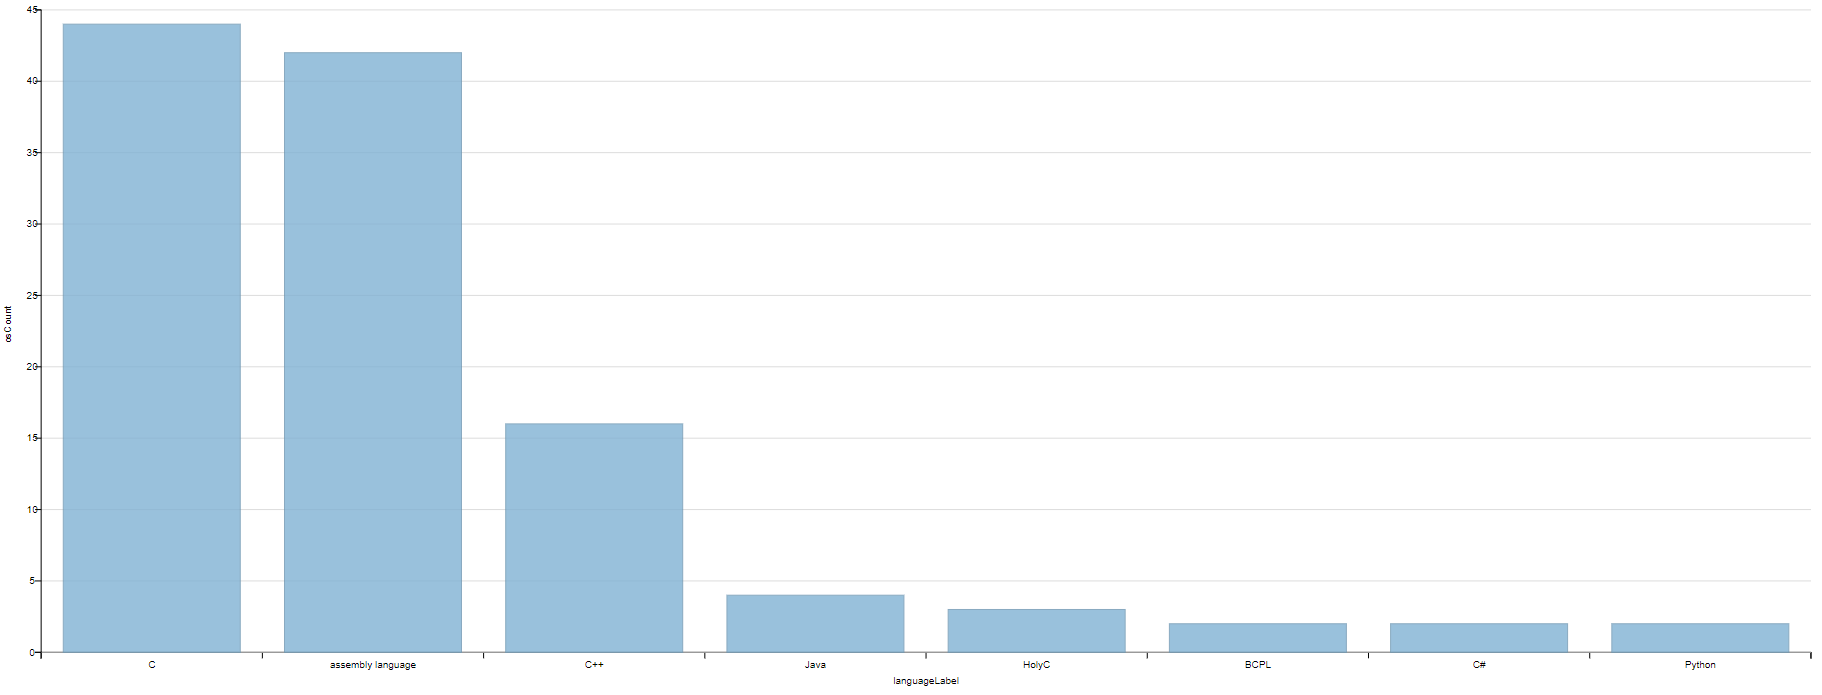
\includegraphics{./chapter/operating_system/count-os-written-on-languages.png}
	\caption{Count of operating systems which written by programming language (2020).}
	\label{fig:count-os-written-on-languages}
\end{figure*}


\begin{figure*}[h!]
	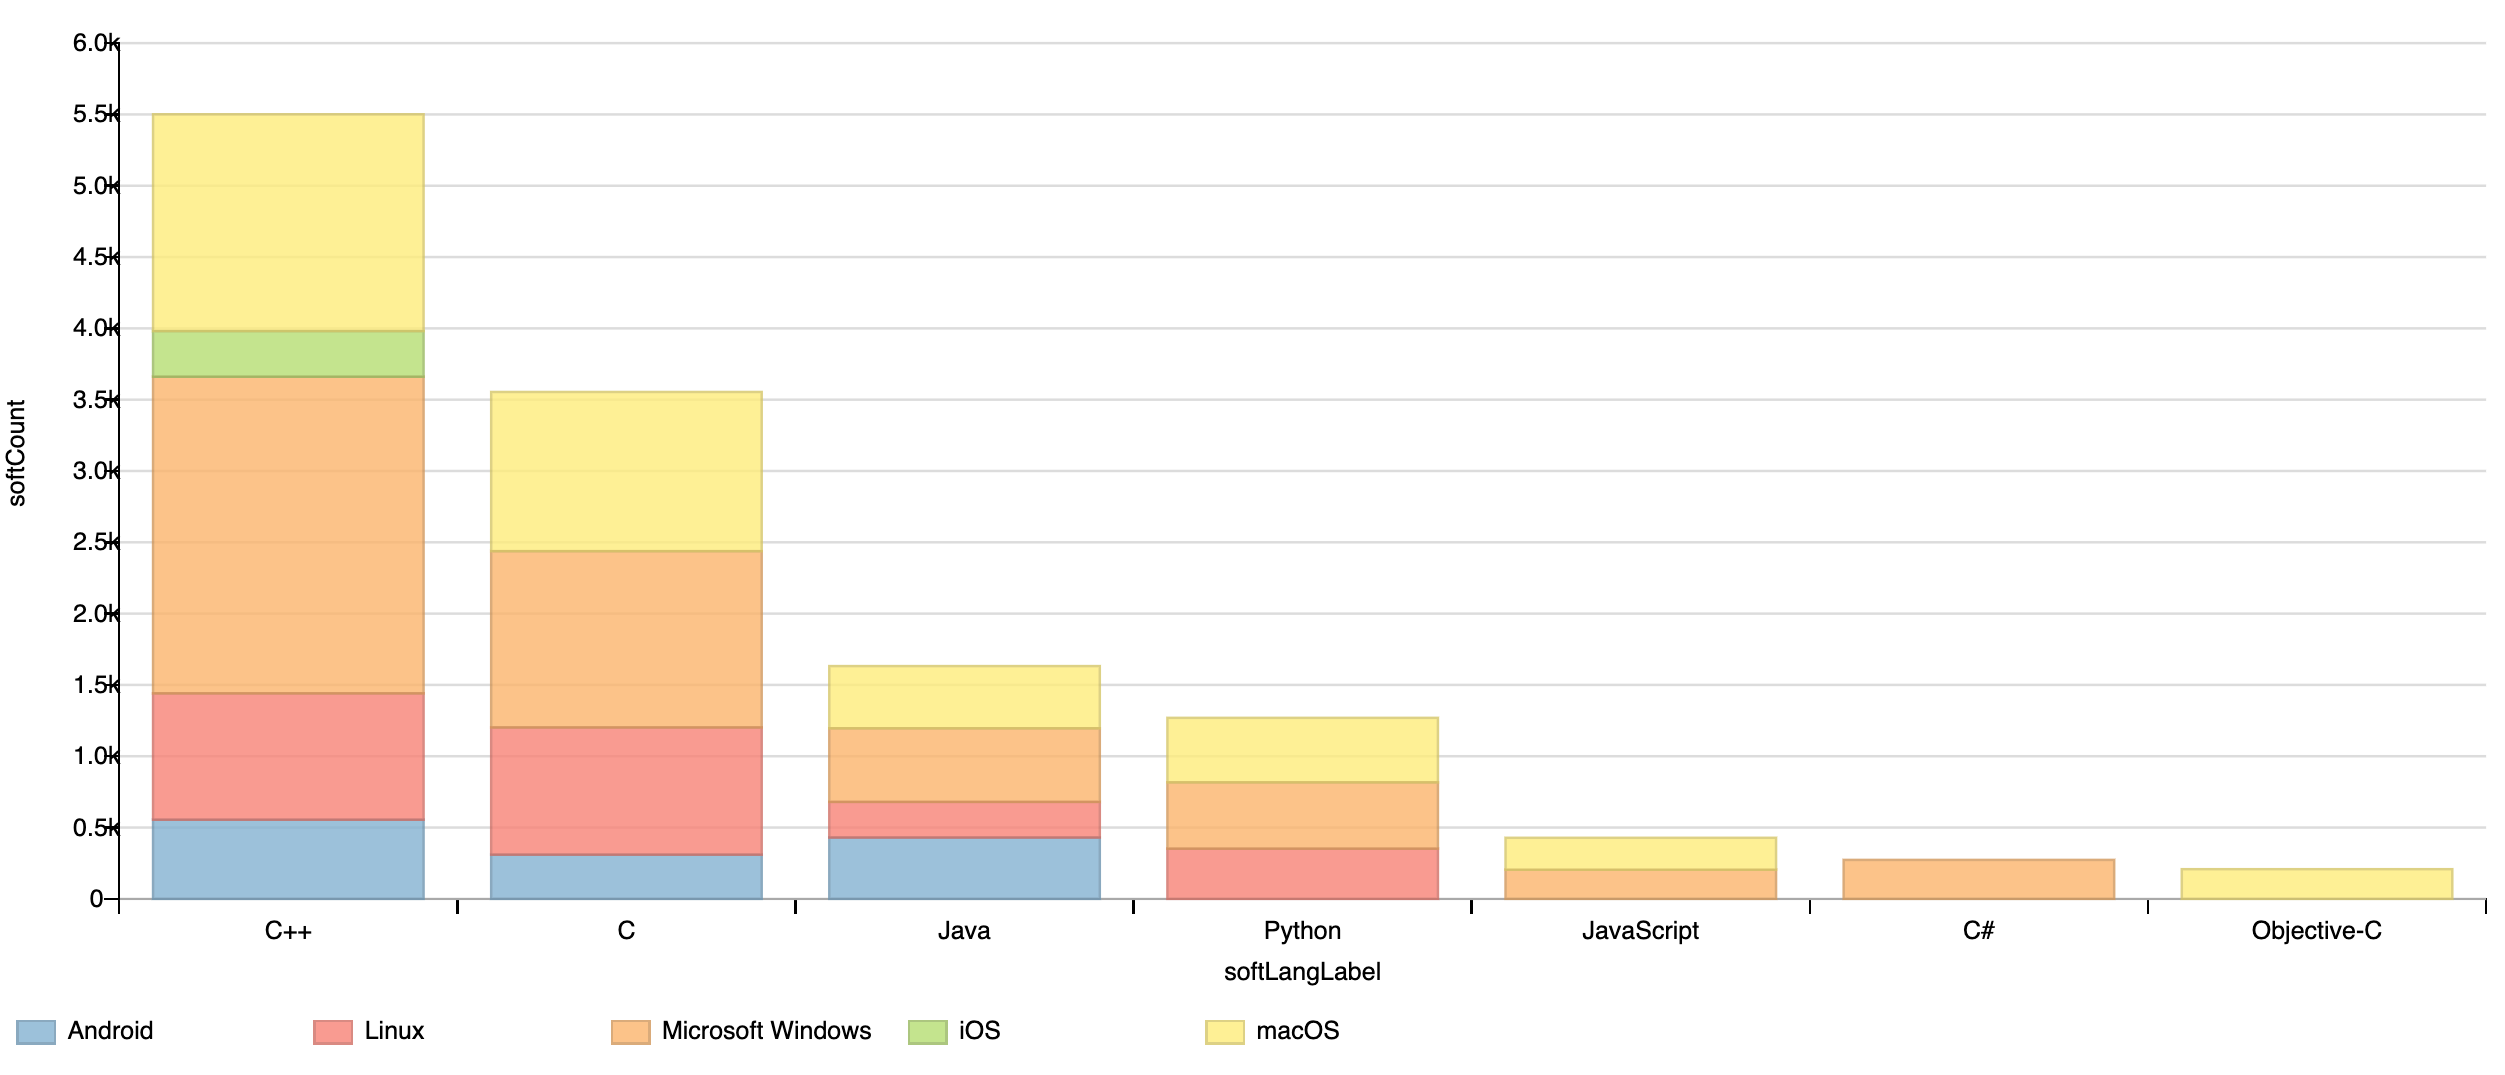
\includegraphics{./chapter/operating_system/Programming-languages-and-count-of-programms-written-on-them-and-OS-2020.png}
	\caption{Programming languages and count of OSs for which programs written in languages (2020).}
	\label{fig:count-software-written-on-languages}
\end{figure*}